\documentclass{standalone}
    \usepackage{tikz}
    \usepackage{amssymb}
    \usetikzlibrary{shapes.geometric, shapes.misc}
    \usetikzlibrary{automata, positioning}

    \begin{document}
    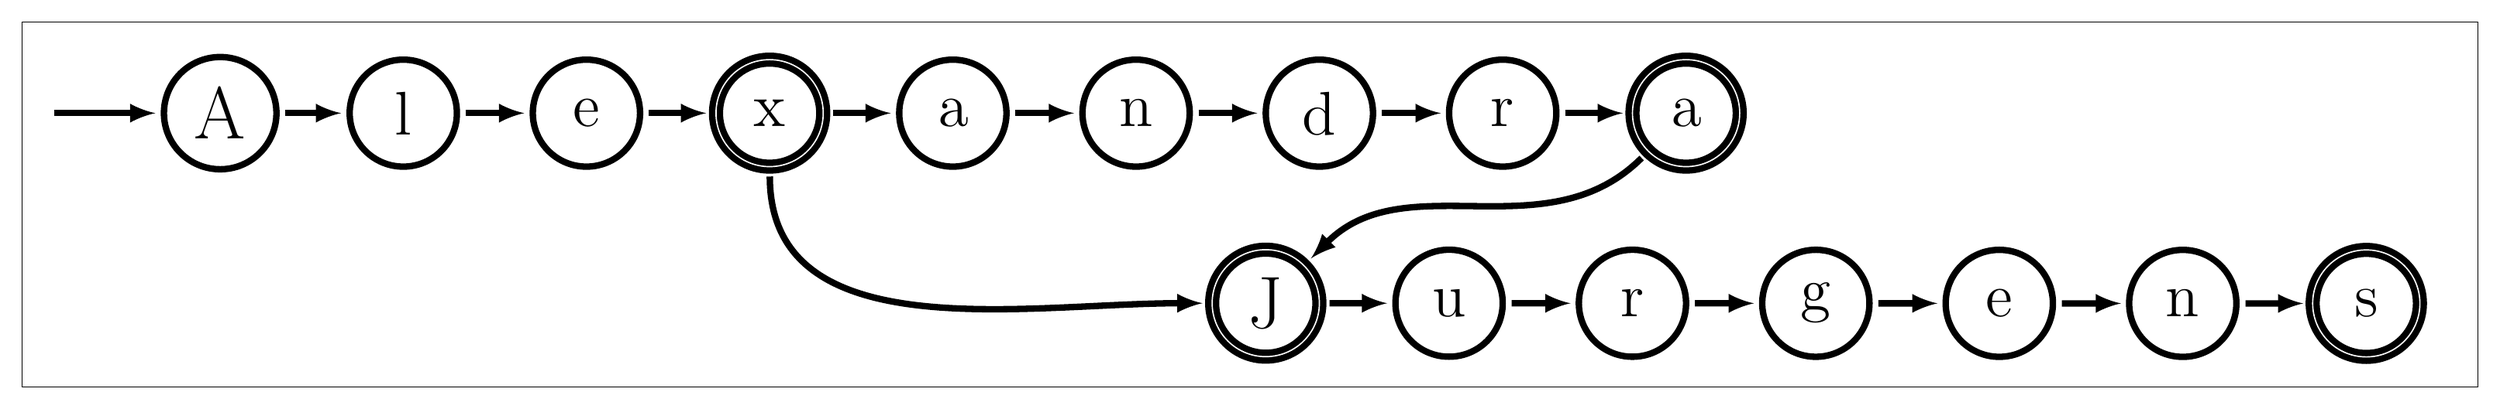
\begin{tikzpicture}[scale=2.5, node distance=1.5cm,
        % bend angle=15, 
        auto,
        every node/.style={scale=2},
        every loop/.style={},
        %,line width=1.2
        every edge/.style={->,draw=black,>=latex,shorten <=1pt, shorten >=1pt},
        every state/.style={draw=black,line width=3,font=\Large, fill=white},
        loop right/.style={right,out=22,in=-22,loop},
        loop above/.style={above,out=112,in=68,loop},
        loop left/.style={left,out=202,in=158,loop},
        loop below/.style={below,out=292,in=248,loop},
        loop above right/.style={right,out=67,in=23,loop},
        loop above left/.style={left,out=157,in=113,loop},
        loop below left/.style={left,out=247,in=203,loop},
        loop below right/.style={right,out=337,in=293,loop},
        binode/.style={minimum size=1cm,inner sep=0pt},]

        \newcommand\translinewidth{3}
        \definecolor{bgcolor}{RGB}{153, 175, 199}

        \draw [] (-.1, .6) rectangle (16, -1.8);

        \node (start) [] {};
        \node[state] (A) [right of=start] {\LARGE A};
        \node[state] (l) [right of=A] {l};
        \node[state] (e) [right of=l] {e};
        \node[state, accepting] (x) [right of=e] {x};
        \node[state] (a) [right of=x] {a};
        \node[state] (n) [right of=a] {n};
        \node[state] (d) [right of=n] {d};
        \node[state] (r) [right of=d] {r};
        \node[state, accepting] (a2) [right of=r] {a};

        \node[state, accepting] (J) [below right of=n, yshift=-0.5cm] {\LARGE J};

        \node[state] (u) [right of=J] {u};
        \node[state] (r2) [right of=u] {r};
        \node[state] (g) [right of=r2] {g};
        \node[state] (e2) [right of=g] {e};
        \node[state] (n2) [right of=e2] {n};
        \node[state, accepting] (accept_s) [right of=n2] {s};

        \path[->, line width=\translinewidth] (start) edge [] node {} (A);
        \path[->, line width=\translinewidth] (A) edge [] node {} (l);       
        \path[->, line width=\translinewidth] (l) edge [] node {} (e);
        \path[->, line width=\translinewidth] (e) edge [] node {} (x);     
        \path[->, line width=\translinewidth] (x) edge [out=270, in=180] node {} (J);
        \path[->, line width=\translinewidth] (x) edge [] node {} (a); 
        \path[->, line width=\translinewidth] (a) edge [] node {} (n);       
        \path[->, line width=\translinewidth] (n) edge [] node {} (d);
        \path[->, line width=\translinewidth] (d) edge [] node {} (r);
        \path[->, line width=\translinewidth] (r) edge [] node {} (a2);
        \path[->, line width=\translinewidth] (a2) edge [out=225, in=45] node {} (J); 
        \path[->, line width=\translinewidth] (J) edge [] node {} (u); 
        \path[->, line width=\translinewidth] (u) edge [] node {} (r2);       
        \path[->, line width=\translinewidth] (r2) edge [] node {} (g);
        \path[->, line width=\translinewidth] (g) edge [] node {} (e2);
        \path[->, line width=\translinewidth] (e2) edge [] node {} (n2);
        \path[->, line width=\translinewidth] (n2) edge [] node {} (accept_s);


        % \path[->, line width=1.2] (n_inf) edge [bend left, in=140] node[pos=0.1] {$\square : \frac{1}{2}$} (n_1);
        % \path[->, line width=1.2] (n_inf) edge [loop above] node {$\triangle : \frac{1}{2}$} (n_inf);
        
    \end{tikzpicture}
    \end{document}